% Options for packages loaded elsewhere
\PassOptionsToPackage{unicode}{hyperref}
\PassOptionsToPackage{hyphens}{url}
\PassOptionsToPackage{dvipsnames,svgnames,x11names}{xcolor}
%
\documentclass[
  10pt]{article}

\usepackage{amsmath,amssymb}
\usepackage{iftex}
\ifPDFTeX
  \usepackage[T1]{fontenc}
  \usepackage[utf8]{inputenc}
  \usepackage{textcomp} % provide euro and other symbols
\else % if luatex or xetex
  \usepackage{unicode-math}
  \defaultfontfeatures{Scale=MatchLowercase}
  \defaultfontfeatures[\rmfamily]{Ligatures=TeX,Scale=1}
\fi
\usepackage{lmodern}
\ifPDFTeX\else  
    % xetex/luatex font selection
\fi
% Use upquote if available, for straight quotes in verbatim environments
\IfFileExists{upquote.sty}{\usepackage{upquote}}{}
\IfFileExists{microtype.sty}{% use microtype if available
  \usepackage[]{microtype}
  \UseMicrotypeSet[protrusion]{basicmath} % disable protrusion for tt fonts
}{}
\makeatletter
\@ifundefined{KOMAClassName}{% if non-KOMA class
  \IfFileExists{parskip.sty}{%
    \usepackage{parskip}
  }{% else
    \setlength{\parindent}{0pt}
    \setlength{\parskip}{6pt plus 2pt minus 1pt}}
}{% if KOMA class
  \KOMAoptions{parskip=half}}
\makeatother
\usepackage{xcolor}
\usepackage[paper=a4paper,inner=2.5cm,outer=3.8cm,bindingoffset=.5cm,top=1.5cm,bottom=1.5cm]{geometry}
\setlength{\emergencystretch}{3em} % prevent overfull lines
\setcounter{secnumdepth}{-\maxdimen} % remove section numbering
% Make \paragraph and \subparagraph free-standing
\ifx\paragraph\undefined\else
  \let\oldparagraph\paragraph
  \renewcommand{\paragraph}[1]{\oldparagraph{#1}\mbox{}}
\fi
\ifx\subparagraph\undefined\else
  \let\oldsubparagraph\subparagraph
  \renewcommand{\subparagraph}[1]{\oldsubparagraph{#1}\mbox{}}
\fi

\usepackage{color}
\usepackage{fancyvrb}
\newcommand{\VerbBar}{|}
\newcommand{\VERB}{\Verb[commandchars=\\\{\}]}
\DefineVerbatimEnvironment{Highlighting}{Verbatim}{commandchars=\\\{\}}
% Add ',fontsize=\small' for more characters per line
\usepackage{framed}
\definecolor{shadecolor}{RGB}{241,243,245}
\newenvironment{Shaded}{\begin{snugshade}}{\end{snugshade}}
\newcommand{\AlertTok}[1]{\textcolor[rgb]{0.68,0.00,0.00}{#1}}
\newcommand{\AnnotationTok}[1]{\textcolor[rgb]{0.37,0.37,0.37}{#1}}
\newcommand{\AttributeTok}[1]{\textcolor[rgb]{0.40,0.45,0.13}{#1}}
\newcommand{\BaseNTok}[1]{\textcolor[rgb]{0.68,0.00,0.00}{#1}}
\newcommand{\BuiltInTok}[1]{\textcolor[rgb]{0.00,0.23,0.31}{#1}}
\newcommand{\CharTok}[1]{\textcolor[rgb]{0.13,0.47,0.30}{#1}}
\newcommand{\CommentTok}[1]{\textcolor[rgb]{0.37,0.37,0.37}{#1}}
\newcommand{\CommentVarTok}[1]{\textcolor[rgb]{0.37,0.37,0.37}{\textit{#1}}}
\newcommand{\ConstantTok}[1]{\textcolor[rgb]{0.56,0.35,0.01}{#1}}
\newcommand{\ControlFlowTok}[1]{\textcolor[rgb]{0.00,0.23,0.31}{#1}}
\newcommand{\DataTypeTok}[1]{\textcolor[rgb]{0.68,0.00,0.00}{#1}}
\newcommand{\DecValTok}[1]{\textcolor[rgb]{0.68,0.00,0.00}{#1}}
\newcommand{\DocumentationTok}[1]{\textcolor[rgb]{0.37,0.37,0.37}{\textit{#1}}}
\newcommand{\ErrorTok}[1]{\textcolor[rgb]{0.68,0.00,0.00}{#1}}
\newcommand{\ExtensionTok}[1]{\textcolor[rgb]{0.00,0.23,0.31}{#1}}
\newcommand{\FloatTok}[1]{\textcolor[rgb]{0.68,0.00,0.00}{#1}}
\newcommand{\FunctionTok}[1]{\textcolor[rgb]{0.28,0.35,0.67}{#1}}
\newcommand{\ImportTok}[1]{\textcolor[rgb]{0.00,0.46,0.62}{#1}}
\newcommand{\InformationTok}[1]{\textcolor[rgb]{0.37,0.37,0.37}{#1}}
\newcommand{\KeywordTok}[1]{\textcolor[rgb]{0.00,0.23,0.31}{#1}}
\newcommand{\NormalTok}[1]{\textcolor[rgb]{0.00,0.23,0.31}{#1}}
\newcommand{\OperatorTok}[1]{\textcolor[rgb]{0.37,0.37,0.37}{#1}}
\newcommand{\OtherTok}[1]{\textcolor[rgb]{0.00,0.23,0.31}{#1}}
\newcommand{\PreprocessorTok}[1]{\textcolor[rgb]{0.68,0.00,0.00}{#1}}
\newcommand{\RegionMarkerTok}[1]{\textcolor[rgb]{0.00,0.23,0.31}{#1}}
\newcommand{\SpecialCharTok}[1]{\textcolor[rgb]{0.37,0.37,0.37}{#1}}
\newcommand{\SpecialStringTok}[1]{\textcolor[rgb]{0.13,0.47,0.30}{#1}}
\newcommand{\StringTok}[1]{\textcolor[rgb]{0.13,0.47,0.30}{#1}}
\newcommand{\VariableTok}[1]{\textcolor[rgb]{0.07,0.07,0.07}{#1}}
\newcommand{\VerbatimStringTok}[1]{\textcolor[rgb]{0.13,0.47,0.30}{#1}}
\newcommand{\WarningTok}[1]{\textcolor[rgb]{0.37,0.37,0.37}{\textit{#1}}}

\providecommand{\tightlist}{%
  \setlength{\itemsep}{0pt}\setlength{\parskip}{0pt}}\usepackage{longtable,booktabs,array}
\usepackage{calc} % for calculating minipage widths
% Correct order of tables after \paragraph or \subparagraph
\usepackage{etoolbox}
\makeatletter
\patchcmd\longtable{\par}{\if@noskipsec\mbox{}\fi\par}{}{}
\makeatother
% Allow footnotes in longtable head/foot
\IfFileExists{footnotehyper.sty}{\usepackage{footnotehyper}}{\usepackage{footnote}}
\makesavenoteenv{longtable}
\usepackage{graphicx}
\makeatletter
\def\maxwidth{\ifdim\Gin@nat@width>\linewidth\linewidth\else\Gin@nat@width\fi}
\def\maxheight{\ifdim\Gin@nat@height>\textheight\textheight\else\Gin@nat@height\fi}
\makeatother
% Scale images if necessary, so that they will not overflow the page
% margins by default, and it is still possible to overwrite the defaults
% using explicit options in \includegraphics[width, height, ...]{}
\setkeys{Gin}{width=\maxwidth,height=\maxheight,keepaspectratio}
% Set default figure placement to htbp
\makeatletter
\def\fps@figure{htbp}
\makeatother
% definitions for citeproc citations
\NewDocumentCommand\citeproctext{}{}
\NewDocumentCommand\citeproc{mm}{%
  \begingroup\def\citeproctext{#2}\cite{#1}\endgroup}
\makeatletter
 % allow citations to break across lines
 \let\@cite@ofmt\@firstofone
 % avoid brackets around text for \cite:
 \def\@biblabel#1{}
 \def\@cite#1#2{{#1\if@tempswa , #2\fi}}
\makeatother
\newlength{\cslhangindent}
\setlength{\cslhangindent}{1.5em}
\newlength{\csllabelwidth}
\setlength{\csllabelwidth}{3em}
\newenvironment{CSLReferences}[2] % #1 hanging-indent, #2 entry-spacing
 {\begin{list}{}{%
  \setlength{\itemindent}{0pt}
  \setlength{\leftmargin}{0pt}
  \setlength{\parsep}{0pt}
  % turn on hanging indent if param 1 is 1
  \ifodd #1
   \setlength{\leftmargin}{\cslhangindent}
   \setlength{\itemindent}{-1\cslhangindent}
  \fi
  % set entry spacing
  \setlength{\itemsep}{#2\baselineskip}}}
 {\end{list}}
\usepackage{calc}
\newcommand{\CSLBlock}[1]{\hfill\break\parbox[t]{\linewidth}{\strut\ignorespaces#1\strut}}
\newcommand{\CSLLeftMargin}[1]{\parbox[t]{\csllabelwidth}{\strut#1\strut}}
\newcommand{\CSLRightInline}[1]{\parbox[t]{\linewidth - \csllabelwidth}{\strut#1\strut}}
\newcommand{\CSLIndent}[1]{\hspace{\cslhangindent}#1}

% \usepackage[utf8]{fontenc}
\usepackage[T1]{fontenc}
\usepackage[autostyle=true]{csquotes}
\usepackage[colorinlistoftodos, textsize=tiny]{todonotes} % insertar comentarios y notas
% \usepackage[spanish]{babel}
\usepackage{longtable}
% \usepackage[disable]{todonotes} # descomentar si quieres QUITAR notas y comentarios

% \renewcommand{\chaptername}{\textbf{Capítulo}}
% \renewcommand{\figurename}{\textbf{Figura}}
% \renewcommand{\tablename}{\textbf{Tabla}}
% \renewcommand{\appendixname}{\textbf{Apéndice}}

% \usepackage{acro}[=v2]
\usepackage{acro}

% \acsetup{list/display=all}
% \usepackage{acro}
% \ac \Ac acronym first time
% \acs \Acs short form
% \acl \Acl longform

\acsetup{
	make-links = true,
    patch/longtable=false
	}

\DeclareAcronym{5-ht}{
    short = 5-HT,
    long = Serotonina
}

\DeclareAcronym{mwm}{
	short = MWM,
	long = Laberinto Acuático de Morris
}
% \DeclareAcronym{5-htp}{
%     short = 5-HTP,
%     long = 5-Hidroxitriptófano
% }


%----------------------------------------------------------------------------------------
%	MARGINS
%----------------------------------------------------------------------------------------

% Márgenes para impresión
% \geometry{
% 	headheight=4ex,
% 	includehead,
% 	includefoot
% }

% Márgenes para web
% \geometry{
%     left=2.5cm,
%     right=2.5cm,
%     top=2.5cm,
%     bottom=2.5cm
% }


% \raggedbottom

% \AtBeginDocument{
% \hypersetup{pdftitle=\ttitle} % Set the PDF's title to your title
% \hypersetup{pdfauthor=\authorname} % Set the PDF's author to your name
% \hypersetup{pdfkeywords=\keywordnames} % Set the PDF's keywords to your keywords
% }
\makeatletter
\@ifpackageloaded{tcolorbox}{}{\usepackage[skins,breakable]{tcolorbox}}
\@ifpackageloaded{fontawesome5}{}{\usepackage{fontawesome5}}
\definecolor{quarto-callout-color}{HTML}{909090}
\definecolor{quarto-callout-note-color}{HTML}{0758E5}
\definecolor{quarto-callout-important-color}{HTML}{CC1914}
\definecolor{quarto-callout-warning-color}{HTML}{EB9113}
\definecolor{quarto-callout-tip-color}{HTML}{00A047}
\definecolor{quarto-callout-caution-color}{HTML}{FC5300}
\definecolor{quarto-callout-color-frame}{HTML}{acacac}
\definecolor{quarto-callout-note-color-frame}{HTML}{4582ec}
\definecolor{quarto-callout-important-color-frame}{HTML}{d9534f}
\definecolor{quarto-callout-warning-color-frame}{HTML}{f0ad4e}
\definecolor{quarto-callout-tip-color-frame}{HTML}{02b875}
\definecolor{quarto-callout-caution-color-frame}{HTML}{fd7e14}
\makeatother
\makeatletter
\@ifpackageloaded{caption}{}{\usepackage{caption}}
\AtBeginDocument{%
\ifdefined\contentsname
  \renewcommand*\contentsname{Tabla de contenidos}
\else
  \newcommand\contentsname{Tabla de contenidos}
\fi
\ifdefined\listfigurename
  \renewcommand*\listfigurename{Listado de Figuras}
\else
  \newcommand\listfigurename{Listado de Figuras}
\fi
\ifdefined\listtablename
  \renewcommand*\listtablename{Listado de Tablas}
\else
  \newcommand\listtablename{Listado de Tablas}
\fi
\ifdefined\figurename
  \renewcommand*\figurename{Figura}
\else
  \newcommand\figurename{Figura}
\fi
\ifdefined\tablename
  \renewcommand*\tablename{Tabla}
\else
  \newcommand\tablename{Tabla}
\fi
}
\@ifpackageloaded{float}{}{\usepackage{float}}
\floatstyle{ruled}
\@ifundefined{c@chapter}{\newfloat{codelisting}{h}{lop}}{\newfloat{codelisting}{h}{lop}[chapter]}
\floatname{codelisting}{Listado}
\newcommand*\listoflistings{\listof{codelisting}{Listado de Listados}}
\makeatother
\makeatletter
\makeatother
\makeatletter
\@ifpackageloaded{caption}{}{\usepackage{caption}}
\@ifpackageloaded{subcaption}{}{\usepackage{subcaption}}
\makeatother
\ifLuaTeX
\usepackage[bidi=basic]{babel}
\else
\usepackage[bidi=default]{babel}
\fi
\babelprovide[main,import]{spanish}
% get rid of language-specific shorthands (see #6817):
\let\LanguageShortHands\languageshorthands
\def\languageshorthands#1{}
\ifLuaTeX
  \usepackage{selnolig}  % disable illegal ligatures
\fi
\usepackage{bookmark}

\IfFileExists{xurl.sty}{\usepackage{xurl}}{} % add URL line breaks if available
\urlstyle{same} % disable monospaced font for URLs
\hypersetup{
  pdftitle={El Narcisista Encubierto en el Laboratorio},
  pdfauthor={string},
  pdflang={es},
  colorlinks=true,
  linkcolor={blue},
  filecolor={Maroon},
  citecolor={Blue},
  urlcolor={Blue},
  pdfcreator={LaTeX via pandoc}}

\title{El Narcisista Encubierto en el Laboratorio}

% \programa{Posgrado en Ciencias Biológicas}

% % \facultad{Facultad de mCiencias} % Nombre de la facultad
% 
% +
% \departmento{Biología Experimental} % Nombre del departamento
% 

% % \grado{MAESTRO EN CIENCIAS BIOLÓGICAS}
% 
% % \supervisor{Dr.~Narcissus}
% 
% % \supervisorfac{Thespiae in Boeotia}
% 
% 
% 
% 
% 


% % \author{string}
% 


% 
% % \university{}
% 


% % \group{}
% 

% \setcounter{tocdepth}{3} % The depth to which the document sections are printed to the table of contents

% %   \author{string}{%
%   % 
\begin{document}

% \frontmatter % Use roman page numbering style (i, ii, iii, iv...) for the pre-content pages

\pagestyle{plain} % Default to the plain heading style until the tesis style is called for the body content
\pagenumbering{Roman}% Capital 'R': uppercase Roman numerals
%----------------------------------------------------------------------------------------
%	PORTADA
%----------------------------------------------------------------------------------------

% Primera portada
\begin{titlepage}
    \begin{center}
        \vspace*{-0.2cm} % Ajusta este valor conforme sea necesario
        
        % Logo de la UNAM
        
\includegraphics[width=3.5cm]{ figuras/unam.png }\\[0.5cm]
        
        % Nombre de la Universidad
        {\large \textbf{UNIVERSIDAD NACIONAL AUTÓNOMA DE MÉXICO}}\\[0.4cm]
        
        % Programa de posgrado
        {\large \textbf{\MakeUppercase{Posgrado en Ciencias
Biológicas}}}\\[0.3cm]
        
        % Facultad y área
        {\large \MakeUppercase{Facultad de mCiencias}}\\[0.2cm]
        {\large \MakeUppercase{Biología Experimental}}\\[0.3cm]
        
        % Título de la tesis
        {\Large \textbf{El Narcisista Encubierto en el
Laboratorio}}\\[0.2cm]
        {\small  Cuando el Perfeccionista Sabotea el Método
Científico }\\[0.2cm]
        
        % Texto "Tesis"
        {\LARGE \textbf{T E S I S}}\\[0.5cm]
        
        % Texto de grado
        {\large QUE PARA OPTAR POR EL GRADO DE:}\\[0.15cm]
        {\Large \textbf{MAESTRO EN CIENCIAS BIOLÓGICAS}}\\[0.4cm]
        
        % Autor
        {\large PRESENTA:}\\[0.1cm]
        {\LARGE \textbf{Santiago García-Rios}}\\[0.4cm]
        
        % Tutor y comité
        {\small \textbf{TUTOR PRINCIPAL DE TESIS:}}\\
        {\small  Dr.~Narcissus }\\
        {\small  Thespiae in Boeotia }\\[0.5cm]
        
        {\small \textbf{COMITÉ TUTOR:}}\\
        {\small  Dr.~Socrates } {\small  Academy of Athens }\\
        {\small  Dr.~Plato } {\small  Academy of Athens }\\
        
        Lugar y fecha
        \vfill
                {\small \textbf{{Ciudad Universitaria,
CD.MX.} \hfill {today}}}\\
                
    \end{center}
\end{titlepage}



% Primera página de \missingfigure
\newpage
\begin{center}
    \missingfigure[figcolor=white]{\MakeUppercase{\LARGE{Página reservada para Derechos de Autor por parte de la Dirección de Bibliotecas.}}}
\end{center}

% Tercera página de \missingfigure
\newpage
\begin{center}
    \missingfigure{\MakeUppercase{\LARGE{Página reservada para Oficio de Jurado.}}}
\end{center}

% agradecimientos institucionales
\newpage
\input{"preambulo/agradecimientos\_institucionales.tex"}

% agradecimientos personales
\newpage
\input{"preambulo/agradecimientos\_personales.tex"}

% dedicatoria
\newpage
\newpage
\begin{center}
    {\LARGE \textbf{\textsc{Dedicatoria}}}\\[1cm]
    \begin{quote}
        \textit{
            Dedico esta tesis a todos los científicos que luchan contra el narcisismo en la academia, ya sea el de sus colegas o el propio. Que este trabajo les recuerde que la ciencia no es un monólogo, sino una conversación colectiva.
        }
    \end{quote}
    \vspace{1cm}
    \begin{quote}
        \textit{
            Y, por supuesto, a Chuck McGill, por ser el arquetipo perfecto de lo que no debemos ser como científicos.
        }
    \end{quote}
\end{center}

\newpage
\begin{center}
    \missingfigure[figcolor=white]{\MakeUppercase{\LARGE{Página en blanco.}}}
\end{center}


\renewcommand*\contentsname{Tabla de contenidos}
\newpage
\tableofcontents

\newpage


\renewcommand{\listfigurename}{Lista de figuras}
\renewcommand{\listtablename}{Lista de tablas}
\listoffigures
\listoftables

% acronimos
\newpage
\printacronyms[name=Abreviaturas]    

% resumen
\newpage
{\LARGE \textbf{\textsc{Resumen}}}\\[0.5cm]

En este trabajo investigamos el impacto del narcisismo encubierto en la práctica científica. Este tipo de narcisismo se manifiesta a menudo como una aparente obsesión por la perfección, aunque en realidad suele traducirse en un sabotaje pasivo-agresivo del método científico. Analizaremos cómo el narcisismo encubierto, disfrazado de falsa modestia, socava los pilares fundamentales de la ciencia: el pensamiento flexible, la crítica constructiva y la humildad intelectual. Después de todo, la frase "Soy muy brillante, pero el mundo está contra mí" suele significar "Soy insufrible con los demás". 

% abstract
\newpage
Resumen en inglés...


\newpage
\pagenumbering{arabic}
\subsection{Introducción}\label{sec-intro}

Ver \textbf{Apartado}~\ref{sec-intro} para mas información.

\begin{tcolorbox}[enhanced jigsaw, colframe=quarto-callout-tip-color-frame, toprule=.15mm, opacitybacktitle=0.6, arc=.35mm, coltitle=black, title=\textcolor{quarto-callout-tip-color}{\faLightbulb}\hspace{0.5em}{Tip}, breakable, rightrule=.15mm, bottomtitle=1mm, titlerule=0mm, leftrule=.75mm, opacityback=0, colbacktitle=quarto-callout-tip-color!10!white, colback=white, left=2mm, bottomrule=.15mm, toptitle=1mm]

\begin{enumerate}
\def\labelenumi{\roman{enumi}.}
\tightlist
\item
  \textbf{Establecer el territorio de investigación:}

  \begin{itemize}
  \tightlist
  \item
    Describir el estado actual del conocimiento sobre el tema.\\
  \item
    Mostrar la relevancia o importancia del área de estudio.\\
  \item
    Revisar investigaciones previas en el campo.\\
    \textbf{Ejemplos:}\\
  \item
    ``La evidencia sugiere que X es uno de los factores más relevantes
    para\ldots{}''\\
  \item
    ``Investigaciones previas han demostrado que\ldots{}''
  \end{itemize}
\item
  \textbf{Identificar un nicho:}

  \begin{itemize}
  \tightlist
  \item
    Motivar la realización del estudio destacando aspectos no abordados
    o problemáticos.\\
  \item
    Esto puede incluir:

    \begin{enumerate}
    \def\labelenumii{\alph{enumii})}
    \tightlist
    \item
      Señalar errores o limitaciones en investigaciones anteriores.\\
    \item
      Resaltar vacíos en el campo.\\
    \item
      Plantear preguntas sin respuesta.\\
    \item
      Proponer contribuciones novedosas.\\
      \textbf{Ejemplos:}\\
    \end{enumerate}
  \item
    ``El análisis de Smith no considera\ldots{}''\\
  \item
    ``Hasta ahora, los estudios sobre X no han abordado\ldots{}''
  \end{itemize}
\item
  \textbf{Ocupar el nicho:}

  \begin{itemize}
  \tightlist
  \item
    Explicar cómo la investigación aborda el problema identificado.\\
  \item
    Definir objetivos, hipótesis o preguntas de investigación.\\
  \item
    Resaltar el valor y la novedad del estudio.\\
  \item
    Describir la estructura del artículo.\\
    \textbf{Ejemplos:}\\
  \item
    ``El propósito de esta investigación es explorar la relación
    entre\ldots{}''\\
  \item
    ``Este estudio proporciona nuevas perspectivas sobre\ldots{}''\\
  \item
    ``El artículo se divide en cuatro secciones\ldots{}''
  \end{itemize}
\end{enumerate}

Estilo narrativo: Expositivo y conciso. Evita detalles técnicos
profundos.

Gramática: Usa presente para hechos establecidos (ej.: ``La plasticidad
neuronal es fundamental para\ldots{}'') y pasado para mencionar
hallazgos previos (ej.: ``Estudios demostraron que\ldots{}'').

\end{tcolorbox}

En este trabajo investigamos el impacto del narcisismo encubierto en la
práctica científica. Este tipo de narcisismo se manifiesta a menudo como
una aparente obsesión por la perfección, aunque en realidad suele
traducirse en un sabotaje pasivo-agresivo del método científico.
Analizaremos cómo el narcisismo encubierto, disfrazado de falsa
modestia, socava los pilares fundamentales de la ciencia: el pensamiento
flexible, la crítica constructiva y la humildad intelectual. Después de
todo, la frase ``Soy muy brillante, pero el mundo está contra mí'' suele
significar ``Soy insufrible con los demás''. Entonces es \ac{5-ht} y
\ac{mwm} y \ac{5-ht} y \ac{mwm}.

Para ilustrar mejor el fenómeno, pensemos en esa persona que publica
``Ugh, odio ser tan inteligente en un mundo de idiotas'' en Facebook
mientras bebe vino de una botella que parece arte contemporáneo y
escucha ``mejor música que la tuya''. Este es el narcisismo encubierto
en acción: el arte de disfrazar la autoimportancia bajo el manto de la
falsa modestia. Exploraremos cómo el cerebro de estos individuos
transforma la autocrítica en un humblebrag (autoelogio disfrazado de
queja) y por qué sus redes neuronales parecen estar organizando un
festival de cine en su propio honor.

\subsubsection{Ejemplos de Narcisismo
Encubierto}\label{ejemplos-de-narcisismo-encubierto}

En general, el narcisismo encubierto se caracteriza por una combinación
de victimización, autoimagen grandiosa y sabotaje pasivo-agresivo
(\textbf{Tabla}~\ref{tbl-actitudes}).

\begin{longtable}[]{@{}
  >{\centering\arraybackslash}p{(\columnwidth - 2\tabcolsep) * \real{0.3933}}
  >{\centering\arraybackslash}p{(\columnwidth - 2\tabcolsep) * \real{0.6067}}@{}}
\caption{Actitudes y Consecuencias del
Narcisista}\label{tbl-actitudes}\tabularnewline
\toprule\noalign{}
\begin{minipage}[b]{\linewidth}\centering
Actitud Narcisista
\end{minipage} & \begin{minipage}[b]{\linewidth}\centering
Consecuencias
\end{minipage} \\
\midrule\noalign{}
\endfirsthead
\toprule\noalign{}
\begin{minipage}[b]{\linewidth}\centering
Actitud Narcisista
\end{minipage} & \begin{minipage}[b]{\linewidth}\centering
Consecuencias
\end{minipage} \\
\midrule\noalign{}
\endhead
\bottomrule\noalign{}
\endlastfoot
``Sufro por ser tan bueno en esto'' & Rechazo a metodologías rigurosas
(ej: Theranos). \\
``Las críticas son envidia'' & Cámaras de eco que perpetúan errores. \\
Autoimagen de mártir & Sabotaje de colaboraciones científicas. \\
Manipulación pasivo-agresiva & Desinformación pública (ej: Goop, teorías
sin base). \\
\end{longtable}

\begin{tcolorbox}[enhanced jigsaw, colframe=quarto-callout-color-frame, toprule=.15mm, leftrule=.75mm, opacityback=0, arc=.35mm, colback=white, bottomrule=.15mm, left=2mm, breakable, rightrule=.15mm]

\vspace{-3mm}\textbf{Chuck McGill (Better Call Saul), caso de estudio}\vspace{3mm}

\textbf{Superioridad y grandiosidad}: Chuck
(\textbf{Fig}~\ref{fig-chuck}) se creía intelectualmente superior a los
demás, especialmente a su hermano Jimmy. Menospreciaba los logros de
Jimmy y lo consideraba moralmente inferior como un mecanismo de defensa
para proteger su autoimagen. Su narcisismo encubierto lo llevó a la
ruina personal y profesional.

\textbf{Necesidad de admiración}: Aunque no lo demostraba abiertamente,
Chuck necesitaba la validación y admiración de los demás. Su ego se
alimentaba de ser reconocido como un abogado brillante y exitoso.

\textbf{Manipulación}: Chuck utilizaba su posición para manipular a los
demás y conseguir lo que quería. Era un maestro en el arte de la
manipulación emocional, haciendo sentir culpables a quienes lo rodeaban.

\textbf{Resentimiento}: Chuck sentía un profundo resentimiento hacia
Jimmy por su éxito y carisma naturales. Este resentimiento lo consumía y
lo llevaba a sabotear los logros de su hermano.

\textbf{Victimización}: A pesar de ser el victimario, Chuck se
presentaba como la víctima. Utilizaba su falsa enfermedad
(hipersensibilidad electromagnética) para manipular a los demás y
obtener simpatía.

\begin{figure}[H]

\centering{

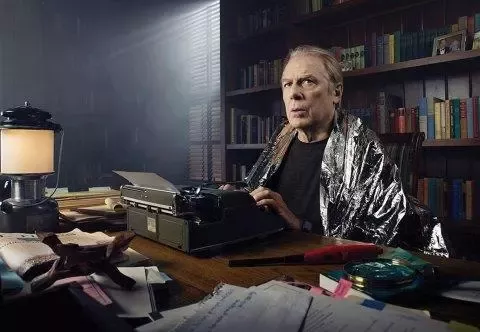
\includegraphics[width=1.6in,height=\textheight]{figuras/chuck.png}

}

\caption{\label{fig-chuck}Chuck McGill fingiendo una enfermedad para
obtener validación de otras personas.}

\end{figure}%

\end{tcolorbox}

\begin{tcolorbox}[enhanced jigsaw, colframe=quarto-callout-important-color-frame, toprule=.15mm, opacitybacktitle=0.6, arc=.35mm, coltitle=black, title=\textcolor{quarto-callout-important-color}{\faExclamation}\hspace{0.5em}{Narcisista Encubierto vs.~Narcisista Evidente}, breakable, rightrule=.15mm, bottomtitle=1mm, titlerule=0mm, leftrule=.75mm, opacityback=0, colbacktitle=quarto-callout-important-color!10!white, colback=white, left=2mm, bottomrule=.15mm, toptitle=1mm]

En la \textbf{Tabla}~\ref{tbl-comparacion}, se presentan las diferencias
clave entre el narcisista encubierto y el narcisista evidente. Mientras
que el narcisista evidente muestra abiertamente su grandiosidad y
necesidad de admiración, el narcisista encubierto lo hace de manera más
sutil, a través de la victimización y la manipulación pasiva.

\begin{longtable}[]{@{}
  >{\raggedright\arraybackslash}p{(\columnwidth - 4\tabcolsep) * \real{0.1341}}
  >{\raggedright\arraybackslash}p{(\columnwidth - 4\tabcolsep) * \real{0.3598}}
  >{\raggedright\arraybackslash}p{(\columnwidth - 4\tabcolsep) * \real{0.5061}}@{}}

\caption{\label{tbl-comparacion}Comparación entre el narcisista
encubierto y el narcisista evidente.}

\tabularnewline

\toprule\noalign{}
\begin{minipage}[b]{\linewidth}\raggedright
Tipo
\end{minipage} & \begin{minipage}[b]{\linewidth}\raggedright
Caracteristicas
\end{minipage} & \begin{minipage}[b]{\linewidth}\raggedright
Ejemplos
\end{minipage} \\
\midrule\noalign{}
\endhead
\bottomrule\noalign{}
\endlastfoot
Narcisista Encubierto & Falsa modestia, victimización, manipulación
pasiva & Chuck McGill (Better Call Saul), `Soy muy brillante, pero el
mundo está contra mí' \\
Narcisista Evidente & Grandiosidad, necesidad de admiración,
manipulación activa & Donald Trump, `Soy el mejor presidente de la
historia, nadie lo hace mejor que yo' \\

\end{longtable}

\end{tcolorbox}

\subsection{Antecedentes}\label{antecedentes}

\begin{tcolorbox}[enhanced jigsaw, colframe=quarto-callout-tip-color-frame, toprule=.15mm, opacitybacktitle=0.6, arc=.35mm, coltitle=black, title=\textcolor{quarto-callout-tip-color}{\faLightbulb}\hspace{0.5em}{Tip}, breakable, rightrule=.15mm, bottomtitle=1mm, titlerule=0mm, leftrule=.75mm, opacityback=0, colbacktitle=quarto-callout-tip-color!10!white, colback=white, left=2mm, bottomrule=.15mm, toptitle=1mm]

Contenido: Revisión crítica de estudios previos, identificando vacíos o
contradicciones que tu trabajo abordará.

Estilo narrativo: Analítico y comparativo. Usa conectores como ``Sin
embargo\ldots{}'', ``A diferencia de\ldots{}''.

Gramática: Tiempos pasados para referirte a investigaciones previas
(ej.: ``X et al.~(2020) observaron que\ldots{}'').

\end{tcolorbox}

(\citeproc{ref-NeurosisEnPijama2023}{2.0, 2023};
\citeproc{ref-IAyNarcisismo2024}{ChatGPT-10, 2024};
\citeproc{ref-FreudRecargado2023}{EgoMeter y BrainDrama, 2023};
\citeproc{ref-DopaminaYSelfies2019}{González y Likeador, 2019};
\citeproc{ref-NeuroFilter2020}{Hashtag, 2020};
\citeproc{ref-SelfieCerebral2022}{Postureo y HumildeFalsa, 2022};
\citeproc{ref-DejaDeLeer2021}{TerapiaExpress, 2021})

(\citeproc{ref-CienciaToxica2024}{Butterfly, 2024};
\citeproc{ref-PopperLloruxf3n2022}{Falsacionista, 2022};
\citeproc{ref-EgoLab2023}{PeerReviewHater y DataCherryPicker, 2023};
\citeproc{ref-AlgorithmShade2024}{Sarcasmo, 2024})

(\citeproc{ref-HolmesFraude2021}{Carreyrou, 2015};
\citeproc{ref-McGillCaseStudy}{Peter Gould, 2015-\/-2022})

\subsection{Planteamiento del
problema}\label{planteamiento-del-problema}

\begin{tcolorbox}[enhanced jigsaw, colframe=quarto-callout-tip-color-frame, toprule=.15mm, opacitybacktitle=0.6, arc=.35mm, coltitle=black, title=\textcolor{quarto-callout-tip-color}{\faLightbulb}\hspace{0.5em}{Tip}, breakable, rightrule=.15mm, bottomtitle=1mm, titlerule=0mm, leftrule=.75mm, opacityback=0, colbacktitle=quarto-callout-tip-color!10!white, colback=white, left=2mm, bottomrule=.15mm, toptitle=1mm]

Contenido: Formula la pregunta de investigación de manera clara y
específica. Ejemplo: ``¿Cómo afecta la exposición a estrés crónico a la
neurogénesis en el hipocampo?''.

Estilo narrativo: Directo y enfocado. Evita ambigüedades.

Gramática: Usa interrogativas directas o frases
declarati\textgreater vas (ej.: ``Se desconoce si\ldots{}'').

\end{tcolorbox}

\begin{quote}
¿Cómo afecta el narcisismo encubierto a la práctica científica? Estos
individuos suelen:
\end{quote}

\begin{itemize}
\tightlist
\item
  Descartar críticas como ``envidia académica''.
\item
  Adulterar datos para que coincidan con su ``brillante intuición''.
\item
  Desacreditar colegas con frases como ``Su metodología es\ldots{}
  interesante'' (traducción: ``Odio que tenga razón'').
\item
  ¿Es posible hacer ciencia rigurosa cuando tu cerebro interpreta
  ``revisión por pares'' como ``ataque personal''?
\end{itemize}

\begin{quote}
¿Cómo detectar a un narcisista encubierto antes de que te invite a su
monólogo sobre lo ``difícil que es ser tan inteligente y sensible''?
\end{quote}

La neurociencia sugiere que sus cerebros podrían tener áreas
hiperactivas en la corteza prefrontal (responsable de la autoevaluación)
y una amígdala que grita ``¡Mírame!'' cada vez que alguien recibe más
likes. ¿Es esto evolución o un bug cerebral?

\subsection{Justificación}\label{justificaciuxf3n}

\begin{tcolorbox}[enhanced jigsaw, colframe=quarto-callout-tip-color-frame, toprule=.15mm, opacitybacktitle=0.6, arc=.35mm, coltitle=black, title=\textcolor{quarto-callout-tip-color}{\faLightbulb}\hspace{0.5em}{Tip}, breakable, rightrule=.15mm, bottomtitle=1mm, titlerule=0mm, leftrule=.75mm, opacityback=0, colbacktitle=quarto-callout-tip-color!10!white, colback=white, left=2mm, bottomrule=.15mm, toptitle=1mm]

Justificación

Contenido: Explica por qué el problema es relevante científicamente,
clínicamente o socialmente. Incluye posibles aplicaciones.

Estilo narrativo: Persuasivo. Destaca el impacto potencial (ej.: ``Este
estudio podría mejorar estrategias para\ldots{}'').

Gramática: Usa futuro hipotético (``podría contribuir a\ldots{}'') y
presente para realidades establecidas (``El estrés es un problema de
salud pública'').

\end{tcolorbox}

Estudiar esto es urgente porque:

\begin{itemize}
\tightlist
\item
  La ciencia no es un monólogo, pero el narcisista encubierto la trata
  como su TED Talk personal.
\item
  El sesgo de confirmación se vuelve dogma cuando el investigador cree
  que ``mi teoría es tan obvia que hasta mi perro la entiende''.
\item
  La reputación de la ciencia se daña cuando los papers incluyen
  ``Agradezco a nadie, porque yo lo hice todo'' en la sección de
  acknowledgments.
\item
  Evitar que la palabra ``humildad'' sea secuestrada por narcisistas.
\item
  Diseñar apps que detecten mensajes pasivo-agresivos en redes sociales
  (``NeuroFilter: ¿Seguro que quieres publicar eso?'').
\item
  Salvar a la humanidad de conversaciones que empiezan con ``Soy
  demasiado empático, es mi maldición''
\end{itemize}

\subsection{Objetivos}\label{objetivos}

\begin{tcolorbox}[enhanced jigsaw, colframe=quarto-callout-tip-color-frame, toprule=.15mm, opacitybacktitle=0.6, arc=.35mm, coltitle=black, title=\textcolor{quarto-callout-tip-color}{\faLightbulb}\hspace{0.5em}{Tip}, breakable, rightrule=.15mm, bottomtitle=1mm, titlerule=0mm, leftrule=.75mm, opacityback=0, colbacktitle=quarto-callout-tip-color!10!white, colback=white, left=2mm, bottomrule=.15mm, toptitle=1mm]

\begin{enumerate}
\def\labelenumi{\arabic{enumi}.}
\setcounter{enumi}{4}
\item
  Objetivos

  Contenido:

\begin{verbatim}
 Objetivo general: Amplio y alineado con el problema.

 Objetivos específicos: Medibles y secuenciales.
\end{verbatim}

  Estilo narrativo: Imperativo o infinitivo (ej.:
  ``Determinar\ldots{}'', ``Analizar\ldots{}'').

  Gramática: Verbos de acción claros (evita ``estudiar'' si es vago; usa
  ``cuantificar'', ``comparar'')
\end{enumerate}

\end{tcolorbox}

\begin{enumerate}
\def\labelenumi{\roman{enumi}.}
\item
  Correlacionar puntuaciones de narcisismo encubierto con resistencia a
  la revisión por pares.
\item
  Cuantificar la frecuencia de frases pasivo-agresivas en correos de
  rechazo a colaboradores (``Lamento que no hayas entendido mi
  genialidad'').
\item
  Demostrar que su corteza prefrontal prioriza ``proteger mi ego'' sobre
  ``aceptar evidencia'' mediante fMRI durante discusiones académicas.
\item
  Desarrollar un algoritmo que detecte narcisismo encubierto en reviews
  anónimos (pista: busca la palabra ``claramente'' seguida de un insulto
  elegante).
\item
  Medir la actividad de la dopamina cuando alguien les dice ``Wow, eres
  tan auténtico''.
\end{enumerate}

\subsection{Hipótesis}\label{hipuxf3tesis}

\begin{tcolorbox}[enhanced jigsaw, colframe=quarto-callout-tip-color-frame, toprule=.15mm, opacitybacktitle=0.6, arc=.35mm, coltitle=black, title=\textcolor{quarto-callout-tip-color}{\faLightbulb}\hspace{0.5em}{Tip}, breakable, rightrule=.15mm, bottomtitle=1mm, titlerule=0mm, leftrule=.75mm, opacityback=0, colbacktitle=quarto-callout-tip-color!10!white, colback=white, left=2mm, bottomrule=.15mm, toptitle=1mm]

\begin{verbatim}
Contenido: Propuesta verificable que responde al problema. Ejemplo: "La deprivación de sueño reduce la densidad sináptica en la corteza prefrontal".

Estilo narrativo: Afirmativo y basado en teoría. Usa condicionales si es exploratorio (ej.: "Se hipotetiza que...").

Gramática: Presente o futuro simple (ej.: "Los ratones expuestos mostrarán...").
\end{verbatim}

Hipótesis: No formularla como pregunta ni incluir metodología

Es un error común formular la \textbf{hipótesis} como una
\textbf{pregunta} porque, por definición, una hipótesis es una
\textbf{afirmación o proposición} que se plantea como una posible
respuesta a la pregunta de investigación. La hipótesis no es la pregunta
en sí, sino una \textbf{predicción fundamentada} que se deriva de la
teoría y los antecedentes, y que será sometida a prueba mediante la
investigación. A continuación, te explico con más detalle por qué es
importante evitar este error:

\begin{center}\rule{0.5\linewidth}{0.5pt}\end{center}

\subsubsection{\texorpdfstring{\textbf{1. La hipótesis es una
afirmación, no una
pregunta}}{1. La hipótesis es una afirmación, no una pregunta}}\label{la-hipuxf3tesis-es-una-afirmaciuxf3n-no-una-pregunta}

\begin{itemize}
\tightlist
\item
  \textbf{Razón científica}: La hipótesis debe ser una declaración que
  pueda ser \textbf{verificada o refutada} empíricamente. Si se formula
  como pregunta, no cumple con este requisito, ya que una pregunta no
  puede ser probada directamente.

  \begin{itemize}
  \tightlist
  \item
    \textbf{Correcto}: \emph{``La exposición a luz azul antes de dormir
    reduce la calidad del sueño en adultos jóvenes.''}\\
  \item
    \textbf{Incorrecto}: \emph{``¿La exposición a luz azul antes de
    dormir reduce la calidad del sueño en adultos jóvenes?''}
  \end{itemize}
\item
  \textbf{Razón narrativa}: La pregunta corresponde al
  \textbf{planteamiento del problema}, no a la hipótesis. La hipótesis
  es el siguiente paso lógico, donde propones una respuesta tentativa
  basada en la teoría y los antecedentes.
\end{itemize}

\begin{center}\rule{0.5\linewidth}{0.5pt}\end{center}

\subsubsection{\texorpdfstring{\textbf{2. La hipótesis debe ser clara y
específica}}{2. La hipótesis debe ser clara y específica}}\label{la-hipuxf3tesis-debe-ser-clara-y-especuxedfica}

\begin{itemize}
\tightlist
\item
  Al formularla como pregunta, se pierde la claridad y precisión que
  requiere una hipótesis científica. Una hipótesis bien formulada debe
  incluir las \textbf{variables} involucradas y la \textbf{relación
  esperada} entre ellas.

  \begin{itemize}
  \tightlist
  \item
    \textbf{Correcto}: \emph{``El aumento en los niveles de cortisol
    está asociado con una disminución en el volumen del hipocampo.''}\\
  \item
    \textbf{Incorrecto}: \emph{``¿El aumento en los niveles de cortisol
    está asociado con una disminución en el volumen del hipocampo?''}
  \end{itemize}
\end{itemize}

\begin{center}\rule{0.5\linewidth}{0.5pt}\end{center}

\subsubsection{\texorpdfstring{\textbf{3. La hipótesis guía el diseño
metodológico}}{3. La hipótesis guía el diseño metodológico}}\label{la-hipuxf3tesis-guuxeda-el-diseuxf1o-metodoluxf3gico}

\begin{itemize}
\tightlist
\item
  Una hipótesis clara y afirmativa permite diseñar métodos específicos
  para probarla. Si es una pregunta, no queda claro qué se está poniendo
  a prueba.

  \begin{itemize}
  \tightlist
  \item
    \textbf{Ejemplo}: Si la hipótesis es \emph{``El estrés crónico
    reduce la neurogénesis en el hipocampo''}, puedes diseñar un
    experimento para medir la neurogénesis en sujetos con y sin estrés.
    Si es una pregunta, no sabes qué relación estás evaluando.
  \end{itemize}
\end{itemize}

\begin{center}\rule{0.5\linewidth}{0.5pt}\end{center}

\subsubsection{\texorpdfstring{\textbf{4. La hipótesis refleja el
enfoque
teórico}}{4. La hipótesis refleja el enfoque teórico}}\label{la-hipuxf3tesis-refleja-el-enfoque-teuxf3rico}

\begin{itemize}
\tightlist
\item
  La hipótesis debe estar basada en la teoría y los antecedentes. Al
  formularla como afirmación, demuestras que has analizado la literatura
  y propones una predicción fundamentada. Si es una pregunta, no se
  evidencia este proceso.

  \begin{itemize}
  \tightlist
  \item
    \textbf{Correcto}: \emph{``Basado en estudios previos, se hipotetiza
    que la deprivación de sueño altera la conectividad funcional en la
    red neuronal por defecto.''}\\
  \item
    \textbf{Incorrecto}: \emph{``¿La deprivación de sueño altera la
    conectividad funcional en la red neuronal por defecto?''}
  \end{itemize}
\end{itemize}

\begin{center}\rule{0.5\linewidth}{0.5pt}\end{center}

\subsubsection{\texorpdfstring{\textbf{5. Coherencia con el método
científico}}{5. Coherencia con el método científico}}\label{coherencia-con-el-muxe9todo-cientuxedfico}

\begin{itemize}
\tightlist
\item
  El método científico implica \textbf{observar, plantear preguntas,
  formular hipótesis, predecir y probar}. La hipótesis es una
  \textbf{predicción}, no una pregunta. Si la hipótesis se formula como
  pregunta, se rompe la lógica del proceso científico.

  \begin{itemize}
  \tightlist
  \item
    \textbf{Ejemplo}:

    \begin{itemize}
    \tightlist
    \item
      \textbf{Pregunta de investigación}: \emph{``¿Cómo afecta el
      ejercicio aeróbico a la memoria de trabajo?''}\\
    \item
      \textbf{Hipótesis}: \emph{``El ejercicio aeróbico mejora el
      rendimiento en tareas de memoria de trabajo.''}
    \end{itemize}
  \end{itemize}
\end{itemize}

\begin{center}\rule{0.5\linewidth}{0.5pt}\end{center}

\subsubsection{\texorpdfstring{\textbf{Consejos para formular una
hipótesis
correctamente}}{Consejos para formular una hipótesis correctamente}}\label{consejos-para-formular-una-hipuxf3tesis-correctamente}

\begin{enumerate}
\def\labelenumi{\arabic{enumi}.}
\tightlist
\item
  \textbf{Basarse en la teoría}: Usa los antecedentes para justificar tu
  predicción.\\
\item
  \textbf{Ser específica}: Incluye las variables y la relación esperada
  entre ellas.\\
\item
  \textbf{Ser comprobable}: Asegúrate de que pueda ser validada o
  refutada con datos.\\
\item
  \textbf{Usar afirmaciones claras}: Evita preguntas, ambigüedades o
  lenguaje vago.
\end{enumerate}

\begin{center}\rule{0.5\linewidth}{0.5pt}\end{center}

\subsubsection{\texorpdfstring{\textbf{Ejemplo de flujo
correcto}}{Ejemplo de flujo correcto}}\label{ejemplo-de-flujo-correcto}

\begin{enumerate}
\def\labelenumi{\arabic{enumi}.}
\tightlist
\item
  \textbf{Pregunta de investigación}: \emph{``¿Cómo afecta la meditación
  mindfulness a la actividad de la amígdala en personas con
  ansiedad?''}\\
\item
  \textbf{Hipótesis}: \emph{``La práctica de meditación mindfulness
  reduce la actividad de la amígdala en personas con ansiedad.''}
\end{enumerate}

\begin{center}\rule{0.5\linewidth}{0.5pt}\end{center}

En resumen, formular la hipótesis como una pregunta es un error porque
desdibuja su función como \textbf{predicción comprobable} y rompe la
estructura lógica del método científico. Una hipótesis bien formulada
debe ser una \textbf{afirmación clara, específica y basada en teoría}
que guíe tu investigación. ¡Espero que esta explicación te sea útil para
tu tesis! 😊

\end{tcolorbox}

Proponemos que el narcisista encubierto:

\begin{itemize}
\tightlist
\item
  Distorsiona el método científico para validar su autoimagen,
  convirtiendo hipótesis en horóscopos académicos (``Los datos no
  coinciden, pero mi intuición es un don'').
\item
  Usa la sección de conflicto de intereses para listar enemigos.
\item
  Su actividad cerebral al recibir críticas se asemeja a la de alguien
  viendo arder su trofeo de kindergarten.
\end{itemize}

\subsection{Metodolodía}\label{metodoloduxeda}

\begin{quote}
Los sujetos negaron todos los resultados, diciendo ``Yo solo estoy aquí
para ayudar a la ciencia'' (clásico).
\end{quote}

\begin{tcolorbox}[enhanced jigsaw, colframe=quarto-callout-tip-color-frame, toprule=.15mm, opacitybacktitle=0.6, arc=.35mm, coltitle=black, title=\textcolor{quarto-callout-tip-color}{\faLightbulb}\hspace{0.5em}{Tip}, breakable, rightrule=.15mm, bottomtitle=1mm, titlerule=0mm, leftrule=.75mm, opacityback=0, colbacktitle=quarto-callout-tip-color!10!white, colback=white, left=2mm, bottomrule=.15mm, toptitle=1mm]

Contenido: Detalla diseño experimental, sujetos/muestras, técnicas (ej.:
fMRI, PCR), análisis estadístico y ética.

Estilo narrativo: Descriptivo y replicable. Usa pasiva para objetividad
(ej.: ``Se utilizó un diseño doble ciego\ldots{}'').

Gramática: Pasado si el estudio ya se realizó; presente si es una
propuesta

\end{tcolorbox}

\begin{tcolorbox}[enhanced jigsaw, colframe=quarto-callout-note-color-frame, toprule=.15mm, opacitybacktitle=0.6, arc=.35mm, coltitle=black, title=\textcolor{quarto-callout-note-color}{\faInfo}\hspace{0.5em}{Términos Importantes}, breakable, rightrule=.15mm, bottomtitle=1mm, titlerule=0mm, leftrule=.75mm, opacityback=0, colbacktitle=quarto-callout-note-color!10!white, colback=white, left=2mm, bottomrule=.15mm, toptitle=1mm]

\emph{Metodología}: Este término es más amplio y no solo describe los
procedimientos específicos utilizados en el experimento, sino también
las bases teóricas que justifican esos métodos. Incluye una discusión
sobre por qué ciertos métodos son apropiados para la investigación en
cuestión. Si tu sección describe tanto el ``cómo'' (los pasos y
procedimientos) como el ``por qué'' (la justificación de la elección de
esos métodos).

\emph{Diseño Experimental}: Este término se refiere específicamente al
plan estructural de la investigación, cómo se organizan los
experimentos, qué variables se controlan, cómo se asignan los sujetos a
diferentes grupos, etc. Es más específico que ``Método'' y se centra en
la planificación del experimento en sí.

\emph{Método}: Es un término más específico y directo. Se enfoca en los
pasos concretos y técnicas empleadas en la investigación, sin
necesariamente entrar en detalles sobre la justificación teórica de esos
métodos.

\end{tcolorbox}

\begin{tcolorbox}[enhanced jigsaw, colframe=quarto-callout-caution-color-frame, toprule=.15mm, opacitybacktitle=0.6, arc=.35mm, coltitle=black, title=\textcolor{quarto-callout-caution-color}{\faFire}\hspace{0.5em}{Voz Pasiva en Metodología}, breakable, rightrule=.15mm, bottomtitle=1mm, titlerule=0mm, leftrule=.75mm, opacityback=0, colbacktitle=quarto-callout-caution-color!10!white, colback=white, left=2mm, bottomrule=.15mm, toptitle=1mm]

Escribir en pasado, con voz pasiva (\emph{Daniel cocinó una tortilla},
\emph{Una tortilla fue cocinada por Danie}, \emph{Daniel la cocinó},
\emph{América fue colonizada en 1492}, \emph{Se reparan automóviles /Se
espera la renuncia del mandatario}), en contraste de voz activa
(\emph{El presidente pronunció un largo discurso}, \emph{Varios millones
visitan Barcelona cada año})

\begin{longtable}[]{@{}
  >{\raggedright\arraybackslash}p{(\columnwidth - 2\tabcolsep) * \real{0.4516}}
  >{\raggedright\arraybackslash}p{(\columnwidth - 2\tabcolsep) * \real{0.5484}}@{}}
\caption{Ejemplos de Voz Activa y Pasiva}\label{tbl-voz}\tabularnewline
\toprule\noalign{}
\begin{minipage}[b]{\linewidth}\raggedright
\textbf{Voz Activa}
\end{minipage} & \begin{minipage}[b]{\linewidth}\raggedright
\textbf{Voz Pasiva}
\end{minipage} \\
\midrule\noalign{}
\endfirsthead
\toprule\noalign{}
\begin{minipage}[b]{\linewidth}\raggedright
\textbf{Voz Activa}
\end{minipage} & \begin{minipage}[b]{\linewidth}\raggedright
\textbf{Voz Pasiva}
\end{minipage} \\
\midrule\noalign{}
\endhead
\bottomrule\noalign{}
\endlastfoot
El presidente pronunció un largo discurso & Un largo discurso fue
pronunciado por el presidente \\
Varios millones visitan Barcelona cada año & Barcelona es visitada cada
año por varios millones \\
Mi madre horneó una tarta de chocolate & Una tarta de chocolate fue
horneada por mi madre \\
Unos ladrones atracaron el banco & El banco fue atracado por unos
ladrone \\
\end{longtable}

\begin{longtable}[]{@{}ll@{}}
\caption{Verbos en Voz Activa y Pasiva}\label{tbl-verbos}\tabularnewline
\toprule\noalign{}
\textbf{Verbo Activo} & \textbf{Verbo Pasivo} \\
\midrule\noalign{}
\endfirsthead
\toprule\noalign{}
\textbf{Verbo Activo} & \textbf{Verbo Pasivo} \\
\midrule\noalign{}
\endhead
\bottomrule\noalign{}
\endlastfoot
Escribe & Es escrito \\
Escribió & Fue escrito \\
Escribirá & Será escrito \\
Escriba & Sea escrito \\
Han escrito & Han sido escritos \\
\end{longtable}

\end{tcolorbox}

\begin{tcolorbox}[enhanced jigsaw, colframe=quarto-callout-tip-color-frame, toprule=.15mm, opacitybacktitle=0.6, arc=.35mm, coltitle=black, title=\textcolor{quarto-callout-tip-color}{\faLightbulb}\hspace{0.5em}{Animales de Laboratorio}, breakable, rightrule=.15mm, bottomtitle=1mm, titlerule=0mm, leftrule=.75mm, opacityback=0, colbacktitle=quarto-callout-tip-color!10!white, colback=white, left=2mm, bottomrule=.15mm, toptitle=1mm]

Reportar el uso de animales de laboratorio, incluyendo:

\begin{itemize}
\tightlist
\item
  Especie, cepa y número de animales
\item
  Cuidado y monitoreo
\item
  Aprovación de comité de ética
\item
  Intervenciones y pasos utilizados para reducir dolor, sufrimiento y
  distrés.
\item
  Cómo se obtuvo el tamaño de la muestra a priori.
\end{itemize}

\end{tcolorbox}

\subsection{Resultados}\label{resultados}

\subsubsection{Reporte de Animales}\label{reporte-de-animales}

\begin{tcolorbox}[enhanced jigsaw, colframe=quarto-callout-tip-color-frame, toprule=.15mm, opacitybacktitle=0.6, arc=.35mm, coltitle=black, title=\textcolor{quarto-callout-tip-color}{\faLightbulb}\hspace{0.5em}{Tip}, breakable, rightrule=.15mm, bottomtitle=1mm, titlerule=0mm, leftrule=.75mm, opacityback=0, colbacktitle=quarto-callout-tip-color!10!white, colback=white, left=2mm, bottomrule=.15mm, toptitle=1mm]

Contenido: Datos crudos (tablas, gráficos) sin interpretación. Responde
a cada objetivo.

Estilo narrativo: Neutral y factual. Ejemplo: ``El grupo experimental
mostró un 20\% menos de\ldots{}''.

Gramática: Pasado (ej.: ``Se observó una correlación
significativa\ldots{}'').

Resultados vs.~Discusión: No mezclar descripción de datos con
interpretación

\end{tcolorbox}

\subsubsection{Scores de Narcisismo Encubierto correlacionan con rechazo
a
críticas}\label{scores-de-narcisismo-encubierto-correlacionan-con-rechazo-a-cruxedticas}

\begin{verbatim}
[1] "Correlación entre Narcisismo y Rechazo a Críticas: 0.69"
\end{verbatim}

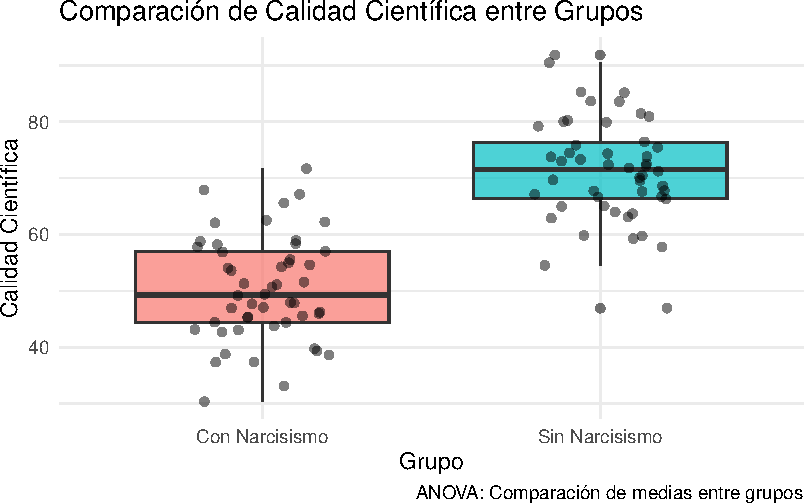
\includegraphics{template_files/figure-pdf/unnamed-chunk-4-1.pdf}

\begin{tcolorbox}[enhanced jigsaw, colframe=quarto-callout-tip-color-frame, toprule=.15mm, opacitybacktitle=0.6, arc=.35mm, coltitle=black, title=\textcolor{quarto-callout-tip-color}{\faLightbulb}\hspace{0.5em}{Tip}, breakable, rightrule=.15mm, bottomtitle=1mm, titlerule=0mm, leftrule=.75mm, opacityback=0, colbacktitle=quarto-callout-tip-color!10!white, colback=white, left=2mm, bottomrule=.15mm, toptitle=1mm]

Puedes usar el paquete de R \texttt{report} (incluido en el código) para
generar automáticamente un informe las pruebas pruebas estadísticas en
formato APA. A pesar que por el momento solo lo hace en inglés, te
ahorrará mucho tiempo y asegura calidad y estandarización de tu reporte.

\begin{verbatim}
Effect sizes were labelled following Funder's (2019) recommendations.

The Pearson's product-moment correlation between datos$Narcisismo and
datos$Rechazo_Criticas is positive, statistically significant, and very large
(r = 0.69, 95% CI [0.57, 0.78], t(98) = 9.33, p < .001)
\end{verbatim}

Y luego puedes incluir el resultado en tu texto:

A mayor narcisismo encubierto, menor citación de colegas en papers r =
0.69, 95\% CI {[}0.57, 0.78{]}, t(98) = 9.33, p \textless{} .001.

\end{tcolorbox}

Correlación entre Narcisismo y Rechazo a Críticas: 0.69

Nivel de narcisismo vs.~Número de veces que dice `La literatura está
equivocada'.

\subsubsection{Activación cerebral en
fMRI}\label{activaciuxf3n-cerebral-en-fmri}

La amígdala se activa un 250\% más al escuchar ``Tu muestra es muy
pequeña'' vs.~``Tu teoría revolucionó la ciencia''.

\begin{Shaded}
\begin{Highlighting}[]
\FunctionTok{install.packages}\NormalTok{(}\StringTok{"fmri"}\NormalTok{)}
\CommentTok{\# devtools::install\_github("muschellij2/fmri")}
\CommentTok{\# https://johnmuschelli.com/Neuroimaging\_in\_R/fmri\_proc.html\#15}
\FunctionTok{library}\NormalTok{(fmri)}

\FunctionTok{source}\NormalTok{(}\StringTok{"https://neuroconductor.org/neurocLite.R"}\NormalTok{)}
\FunctionTok{neuro\_install}\NormalTok{(}\StringTok{"neurobase"}\NormalTok{, }\AttributeTok{release =} \StringTok{"stable"}\NormalTok{)}

\FunctionTok{orthographic}\NormalTok{(data)}
\end{Highlighting}
\end{Shaded}

\subsubsection{Análisis de texto}\label{anuxe1lisis-de-texto}

El 90\% de sus emails incluyen ``Con todo respeto\ldots{}'' seguido de
un ``Pero esto es basura'' disfrazado de citas de Popper.

\begin{verbatim}
             Df Sum Sq Mean Sq F value Pr(>F)    
Grupo         2  14046    7023   97.69 <2e-16 ***
Residuals   147  10568      72                   
---
Signif. codes:  0 '***' 0.001 '**' 0.01 '*' 0.05 '.' 0.1 ' ' 1
\end{verbatim}

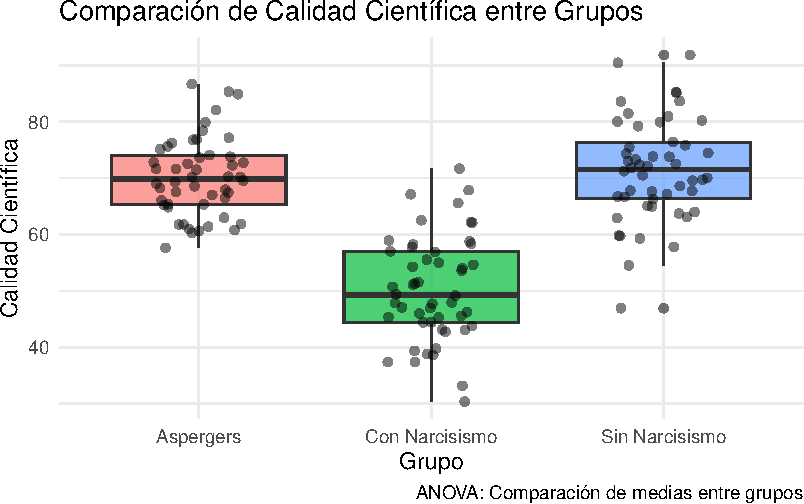
\includegraphics{template_files/figure-pdf/unnamed-chunk-6-1.pdf}

\begin{tcolorbox}[enhanced jigsaw, colframe=quarto-callout-tip-color-frame, toprule=.15mm, opacitybacktitle=0.6, arc=.35mm, coltitle=black, title=\textcolor{quarto-callout-tip-color}{\faLightbulb}\hspace{0.5em}{Tip}, breakable, rightrule=.15mm, bottomtitle=1mm, titlerule=0mm, leftrule=.75mm, opacityback=0, colbacktitle=quarto-callout-tip-color!10!white, colback=white, left=2mm, bottomrule=.15mm, toptitle=1mm]

\begin{verbatim}
The ANOVA (formula: Calidad_Cientifica ~ Grupo) suggests that:

  - The main effect of Grupo is statistically significant and large (F(2, 147) =
97.69, p < .001; Eta2 = 0.57, 95% CI [0.49, 1.00])

Effect sizes were labelled following Field's (2013) recommendations.
\end{verbatim}

\end{tcolorbox}

El ANOVA y el gráfico sugieren que las personas con narcisismo
encubierto tienden a tener una calidad científica significativamente
menor que aquellas sin narcisismo. Esto respalda tu hipótesis de que el
narcisismo encubierto es incompatible con la buena ciencia, ya que
afecta negativamente la capacidad de colaborar, aceptar críticas y
mantener estándares rigurosos.

\subsection{Extra}\label{extra}

\begin{Shaded}
\begin{Highlighting}[]
\NormalTok{p1 }\OtherTok{\textless{}{-}} \FunctionTok{ggplot}\NormalTok{(iris, }\FunctionTok{aes}\NormalTok{(}\AttributeTok{x =}\NormalTok{ Species, }\AttributeTok{y =}\NormalTok{ Sepal.Length, }\AttributeTok{fill =}\NormalTok{ Species)) }\SpecialCharTok{+}
  \FunctionTok{geom\_boxplot}\NormalTok{() }\SpecialCharTok{+}
  \FunctionTok{theme\_modern}\NormalTok{(}\AttributeTok{axis.text.angle =} \DecValTok{45}\NormalTok{) }\SpecialCharTok{+}
  \FunctionTok{scale\_fill\_material\_d}\NormalTok{()}

\NormalTok{p2 }\OtherTok{\textless{}{-}} \FunctionTok{ggplot}\NormalTok{(iris, }\FunctionTok{aes}\NormalTok{(}\AttributeTok{x =}\NormalTok{ Species, }\AttributeTok{y =}\NormalTok{ Sepal.Length, }\AttributeTok{fill =}\NormalTok{ Species)) }\SpecialCharTok{+}
  \FunctionTok{geom\_violin}\NormalTok{() }\SpecialCharTok{+}
  \FunctionTok{theme\_modern}\NormalTok{(}\AttributeTok{axis.text.angle =} \DecValTok{45}\NormalTok{) }\SpecialCharTok{+}
  \FunctionTok{scale\_fill\_material\_d}\NormalTok{(}\AttributeTok{palette =} \StringTok{"ice"}\NormalTok{)}

\NormalTok{p3 }\OtherTok{\textless{}{-}} \FunctionTok{ggplot}\NormalTok{(iris, }\FunctionTok{aes}\NormalTok{(}\AttributeTok{x =}\NormalTok{ Petal.Length, }\AttributeTok{y =}\NormalTok{ Petal.Width, }\AttributeTok{color =}\NormalTok{ Sepal.Length)) }\SpecialCharTok{+}
  \FunctionTok{geom\_point2}\NormalTok{() }\SpecialCharTok{+}
  \FunctionTok{theme\_modern}\NormalTok{() }\SpecialCharTok{+}
  \FunctionTok{scale\_color\_material\_c}\NormalTok{(}\AttributeTok{palette =} \StringTok{"rainbow"}\NormalTok{)}

\FunctionTok{plots}\NormalTok{(p1, p2, p3, }\AttributeTok{n\_columns =} \DecValTok{2}\NormalTok{)}
\end{Highlighting}
\end{Shaded}

\subsection{Discusión}\label{discusiuxf3n}

\begin{tcolorbox}[enhanced jigsaw, colframe=quarto-callout-tip-color-frame, toprule=.15mm, opacitybacktitle=0.6, arc=.35mm, coltitle=black, title=\textcolor{quarto-callout-tip-color}{\faLightbulb}\hspace{0.5em}{Tip}, breakable, rightrule=.15mm, bottomtitle=1mm, titlerule=0mm, leftrule=.75mm, opacityback=0, colbacktitle=quarto-callout-tip-color!10!white, colback=white, left=2mm, bottomrule=.15mm, toptitle=1mm]

\begin{verbatim}
Contenido: Interpreta resultados, contrasta con antecedentes, explica limitaciones y sugiere futuras investigaciones.

Estilo narrativo: Crítico y reflexivo. Usa comparaciones (ej.: "A diferencia de X, nuestros hallazgos sugieren...").

Gramática: Presente para teorías aceptadas (ej.: "Estos datos apoyan la hipótesis de que...").
\end{verbatim}

\end{tcolorbox}

\subsection{Conclusión}\label{conclusiuxf3n}

\begin{tcolorbox}[enhanced jigsaw, colframe=quarto-callout-tip-color-frame, toprule=.15mm, opacitybacktitle=0.6, arc=.35mm, coltitle=black, title=\textcolor{quarto-callout-tip-color}{\faLightbulb}\hspace{0.5em}{Tip}, breakable, rightrule=.15mm, bottomtitle=1mm, titlerule=0mm, leftrule=.75mm, opacityback=0, colbacktitle=quarto-callout-tip-color!10!white, colback=white, left=2mm, bottomrule=.15mm, toptitle=1mm]

Contenido: Síntesis de hallazgos clave y su relevancia. No repitas
resultados.

Estilo narrativo: Conciso y enfocado en contribuciones.

Gramática: Presente perfecto o presente (ej.: ``Este estudio demuestra
que\ldots{}'')

Conclusión: No introducir nuevos datos o ideas no discutidas
previamente.

\end{tcolorbox}

El narcisismo encubierto es el virus silencioso de la mala ciencia:
convierte la duda en herejía, la colaboración en competencia, y los
journals en diarios íntimos con DOI. La solución no es expulsarlos, sino
mandarlos a un retiro espiritual con Carl Sagan de fondo (``El universo
no gira en torno a ti, Karen''). Propuesta: incluir tests de narcisismo
en las convocatorias de financiamiento. Cof cof.

Confirmamos que el narcisismo encubierto es como el ajo en las recetas:
todos creen que no lo usan, pero se huele a kilómetros. La neurociencia
sugiere que sus cerebros son máquinas de autoengaño sofisticadas, pero
con suficiente humor y memes, quizá podamos salvarlos (o al menos
reírnos en el proceso). Propuesta final: un bot de Twitter que responda
``Ok, Sigmund Freud'' a sus hilos existenciales.

\subsection{Apéndices}\label{apuxe9ndices}

\subsubsection{Supuestos Estadísticos}\label{supuestos-estaduxedsticos}

\begin{Shaded}
\begin{Highlighting}[]
\FunctionTok{install.packages}\NormalTok{(}\StringTok{"easystats"}\NormalTok{)}
\FunctionTok{install.packages}\NormalTok{(}\StringTok{"patchwork"}\NormalTok{)}
\FunctionTok{library}\NormalTok{(performance)}
\FunctionTok{library}\NormalTok{(see)}

\NormalTok{model }\OtherTok{\textless{}{-}} \FunctionTok{lm}\NormalTok{(wt }\SpecialCharTok{\textasciitilde{}}\NormalTok{ mpg, }\AttributeTok{data =}\NormalTok{ mtcars)}
\NormalTok{check }\OtherTok{\textless{}{-}} \FunctionTok{check\_normality}\NormalTok{(model)}

\FunctionTok{plot}\NormalTok{(check, }\AttributeTok{type =} \StringTok{"qq"}\NormalTok{)}

\NormalTok{m }\OtherTok{\textless{}{-}} \FunctionTok{lm}\NormalTok{(mpg }\SpecialCharTok{\textasciitilde{}}\NormalTok{ wt }\SpecialCharTok{+}\NormalTok{ cyl }\SpecialCharTok{+}\NormalTok{ gear }\SpecialCharTok{+}\NormalTok{ disp, }\AttributeTok{data =}\NormalTok{ mtcars)}
\NormalTok{result }\OtherTok{\textless{}{-}} \FunctionTok{check\_collinearity}\NormalTok{(m)}

\CommentTok{\# result}

\FunctionTok{plot}\NormalTok{(result)}


\CommentTok{\# select only mpg and disp (continuous)}
\NormalTok{mt1 }\OtherTok{\textless{}{-}}\NormalTok{ mtcars[, }\FunctionTok{c}\NormalTok{(}\DecValTok{1}\NormalTok{, }\DecValTok{3}\NormalTok{, }\DecValTok{4}\NormalTok{)]}
\CommentTok{\# create some fake outliers and attach outliers to main df}
\NormalTok{mt2 }\OtherTok{\textless{}{-}} \FunctionTok{rbind}\NormalTok{(mt1, }\FunctionTok{data.frame}\NormalTok{(}\AttributeTok{mpg =} \FunctionTok{c}\NormalTok{(}\DecValTok{37}\NormalTok{, }\DecValTok{40}\NormalTok{), }\AttributeTok{disp =} \FunctionTok{c}\NormalTok{(}\DecValTok{300}\NormalTok{, }\DecValTok{400}\NormalTok{), }\AttributeTok{hp =} \FunctionTok{c}\NormalTok{(}\DecValTok{110}\NormalTok{, }\DecValTok{120}\NormalTok{)))}
\CommentTok{\# fit model with outliers}
\NormalTok{model }\OtherTok{\textless{}{-}} \FunctionTok{lm}\NormalTok{(disp }\SpecialCharTok{\textasciitilde{}}\NormalTok{ mpg }\SpecialCharTok{+}\NormalTok{ hp, }\AttributeTok{data =}\NormalTok{ mt2)}
\NormalTok{result }\OtherTok{\textless{}{-}} \FunctionTok{check\_outliers}\NormalTok{(model)}

\FunctionTok{plot}\NormalTok{(result, }\AttributeTok{type =} \StringTok{"dots"}\NormalTok{)}

\NormalTok{model2 }\OtherTok{\textless{}{-}} \FunctionTok{lm}\NormalTok{(mpg }\SpecialCharTok{\textasciitilde{}}\NormalTok{ wt }\SpecialCharTok{+}\NormalTok{ cyl }\SpecialCharTok{+}\NormalTok{ gear }\SpecialCharTok{+}\NormalTok{ disp, }\AttributeTok{data =}\NormalTok{ mtcars)}
\NormalTok{result2 }\OtherTok{\textless{}{-}} \FunctionTok{check\_normality}\NormalTok{(model2)}

\FunctionTok{plot}\NormalTok{(result2, }\AttributeTok{type =} \StringTok{"density"}\NormalTok{)}

\FunctionTok{plot}\NormalTok{(result2, }\AttributeTok{type =} \StringTok{"qq"}\NormalTok{)}

\NormalTok{model }\OtherTok{\textless{}{-}} \FunctionTok{lm}\NormalTok{(mpg }\SpecialCharTok{\textasciitilde{}}\NormalTok{ wt }\SpecialCharTok{+}\NormalTok{ cyl }\SpecialCharTok{+}\NormalTok{ gear }\SpecialCharTok{+}\NormalTok{ disp, }\AttributeTok{data =}\NormalTok{ mtcars)}
\NormalTok{result }\OtherTok{\textless{}{-}} \FunctionTok{check\_heteroscedasticity}\NormalTok{(model)}
\FunctionTok{plot}\NormalTok{(result)}
\end{Highlighting}
\end{Shaded}

\subsubsection{Info}\label{info}

\begin{verbatim}
Analyses were conducted using the R Statistical language (version 4.3.1; R Core
Team, 2023) on Ubuntu 22.04.4 LTS, using the packages ggpubr (version 0.6.0;
Kassambara A, 2023), report (version 0.5.7; Makowski D et al., 2023), ggplot2
(version 3.4.4; Wickham H, 2016) and dplyr (version 1.1.3; Wickham H et al.,
2023).

References
----------
  - Kassambara A (2023). _ggpubr: 'ggplot2' Based Publication Ready Plots_. R
package version 0.6.0, <https://rpkgs.datanovia.com/ggpubr/>.
  - Makowski D, Lüdecke D, Patil I, Thériault R, Ben-Shachar M, Wiernik B (2023).
"Automated Results Reporting as a Practical Tool to Improve Reproducibility and
Methodological Best Practices Adoption." _CRAN_.
<https://easystats.github.io/report/>.
  - R Core Team (2023). _R: A Language and Environment for Statistical
Computing_. R Foundation for Statistical Computing, Vienna, Austria.
<https://www.R-project.org/>.
  - Wickham H (2016). _ggplot2: Elegant Graphics for Data Analysis_.
Springer-Verlag New York. ISBN 978-3-319-24277-4,
<https://ggplot2.tidyverse.org>.
  - Wickham H, François R, Henry L, Müller K, Vaughan D (2023). _dplyr: A Grammar
of Data Manipulation_. https://dplyr.tidyverse.org,
https://github.com/tidyverse/dplyr.
\end{verbatim}

\subsection*{Referencias}\label{referencias}
\addcontentsline{toc}{subsection}{Referencias}

\phantomsection\label{refs}
\begin{CSLReferences}{1}{0}
\bibitem[\citeproctext]{ref-NeurosisEnPijama2023}
2.0, F. (2023). \emph{Neurosis en Pijama: La Neurociencia del Que Sube
Historias Motivacionales a las 3 AM}. Silicon Valley: NeuroVanity Press.

\bibitem[\citeproctext]{ref-CienciaToxica2024}
Butterfly, Dr. I. R. (2024). \emph{Ciencia Tóxica: Cuando el Ego es el
Principal {COI} (Conflicto de Intereses)}. Cambridge: Black Hole
Academic Press.

\bibitem[\citeproctext]{ref-HolmesFraude2021}
Carreyrou, J. (2015). Bad Blood: Secrets and Lies in a Silicon Valley
Startup. \emph{The Wall Street Journal}.

\bibitem[\citeproctext]{ref-IAyNarcisismo2024}
ChatGPT-10. (2024). \emph{¿Puede la {IA} Diagnosticar a tu Ex? Un
Análisis de Mensajes Pasivo-Agresivos en Tinder} (Reporte Técnico N.º
NTD-007). Instituto de Tecnologías Dramáticas.

\bibitem[\citeproctext]{ref-FreudRecargado2023}
EgoMeter, V., y BrainDrama, L. (2023). Why Do I Love Me? A Neural Survey
of Self-Admiration. \emph{Journal of Questionable Personality Traits},
\emph{42}(6), 1337-1350. \url{https://doi.org/10.1234/jqpt.2023.007}

\bibitem[\citeproctext]{ref-PopperLloruxf3n2022}
Falsacionista, K. (2022). El Narcisista y la Falsabilidad: Por Qué su
Hipótesis es Inmune a los Hechos. En \emph{Psicopatologías de la Razón:
Filosofía para Científicos con Daddy Issues} (pp. 777-789). Ediciones
Crítica Constructiva (Ironicamente).

\bibitem[\citeproctext]{ref-DopaminaYSelfies2019}
González, D., y Likeador, S. (2019). La Curva de la Dopamina en
Publicaciones de Café Artesanal: Un Estudio con Narcisistas Encubiertos.
\emph{Annual Review of Pretentious Behavior}, \emph{7}, 42-666.
\url{https://doi.org/10.6666/ar.pb.2019.007}

\bibitem[\citeproctext]{ref-NeuroFilter2020}
Hashtag, A. (2020). NeuroFilter: Cómo Detectar un {{«Humblebrag»}} en
280 Caracteres o Menos. En T. Académico (Ed.), \emph{Memes y Neuronas:
La Ciencia detrás de tu Timeline Tóxico} (pp. 69-420). TikTok Academic
Publications.

\bibitem[\citeproctext]{ref-EgoLab2023}
PeerReviewHater, R., y DataCherryPicker, E. (2023). Narcissus in the
Lab: How Covert Narcissism Corrupts Citation Networks. \emph{Journal of
Irreproducible Results}, \emph{12}, 45-69.
\url{https://doi.org/10.6666/jir.2023.045}

\bibitem[\citeproctext]{ref-McGillCaseStudy}
Peter Gould, V. G. y. (2015-\/-2022). \emph{Better Call Saul: Análisis
de Chuck McGill como arquetipo del narcisista encubierto en entornos de
alta exigencia}.

\bibitem[\citeproctext]{ref-SelfieCerebral2022}
Postureo, C., y HumildeFalsa, M. (2022). \emph{Humblebrags \& Brain
Scans: {fMRI} No Miente, Tu Perfil de Instagram Sí} (1st ed.). Berlin:
Springer.

\bibitem[\citeproctext]{ref-AlgorithmShade2024}
Sarcasmo, A. (2024). \emph{Detecting Academic Narcissism via
Passive-Aggressive LaTeX Comments: A Machine Learning Approach}
(Technical Report N.º IDPR-666). Recuperado de Institute of Dramatic
Peer Review website: \url{https://arxiv.org/abs/2404.01joke}

\bibitem[\citeproctext]{ref-DejaDeLeer2021}
TerapiaExpress, A. (2021). \emph{Deja de Leer Esto y Ve a Terapia: Guía
de Supervivencia para el Autoengañado Crónico}. Buenos Aires: Ediciones
Ironía Sana.

\end{CSLReferences}



\end{document}
